\documentclass[pdf]{beamer}
\usepackage[english,vietnamese]{babel}
\usepackage{amsmath}
\usepackage{booktabs}
\usepackage{graphicx}
\usepackage{hyperref}
\usepackage{lmodern}
\usepackage{siunitx}

\mode<presentation>{}
\usetheme[hideothersubsections]{Hannover}
\usecolortheme{crane}
\usefonttheme[onlymath]{serif}
\usebackgroundtemplate{
  
\includegraphics[width=\paperwidth,height=\paperheight]{USTH.jpg}}
\renewcommand{\thefootnote}{\fnsymbol{footnote}}
\setcounter{tocdepth}{2}

\title{Python Package Metadata Management}
\author[Group 8]{Nguyễn Gia Phong---BI9-184\\
                 Nguyễn Quốc Thông---BI9-214\\
                 Nguyễn Văn Tùng---BI9-229\\
                 Trần Minh Vương---BI9-239}
\institute{University of Science and Technology of Hà Nội}
\date{\selectlanguage{english}\today}

\begin{document}
\frame{\titlepage}
\selectlanguage{english}
\begin{frame}{Contents}
  \tableofcontents
\end{frame}

\section{Introduction}
\frame{\tableofcontents[currentsection]}

\section{Conclusion}
\frame{\tableofcontents[currentsection]}
\begin{frame}{Copying}\Large
  \begin{center}
    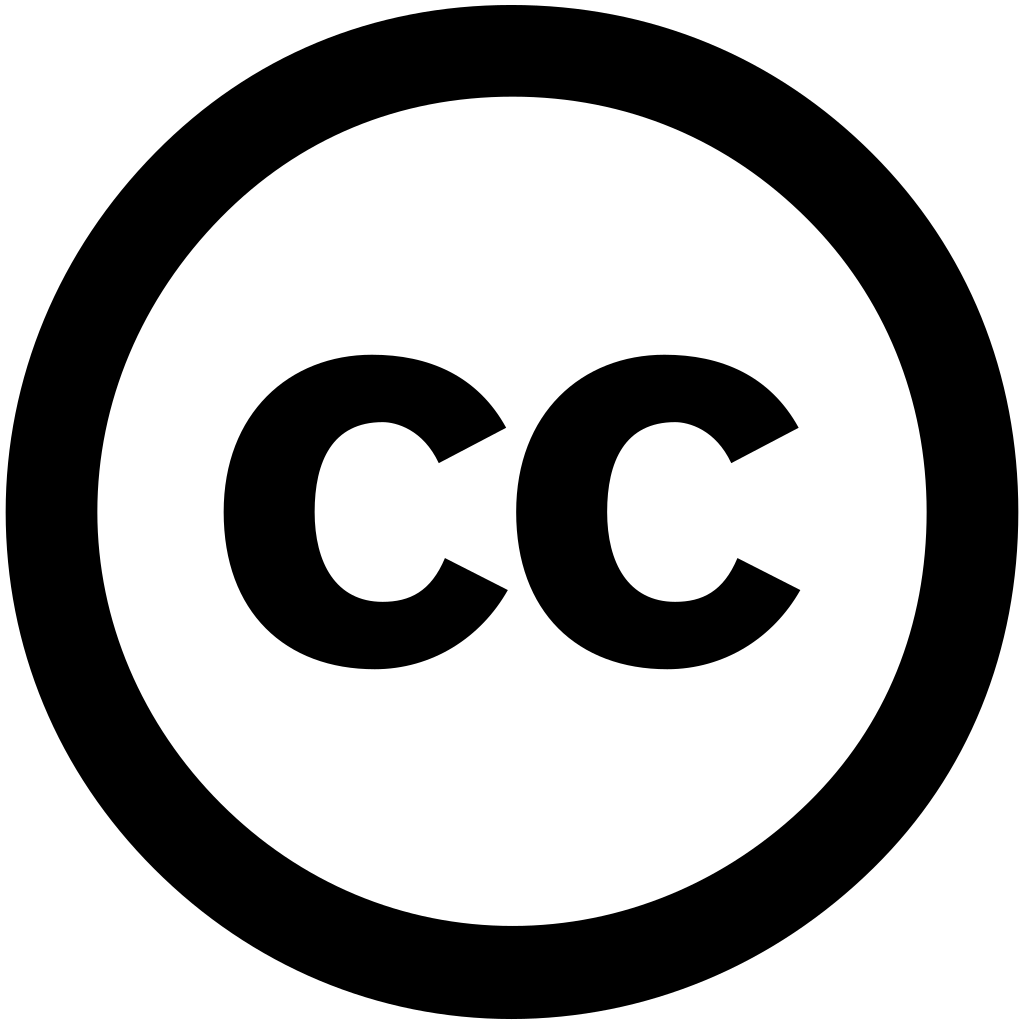
\includegraphics[width=0.2\textwidth]{CC.png}
    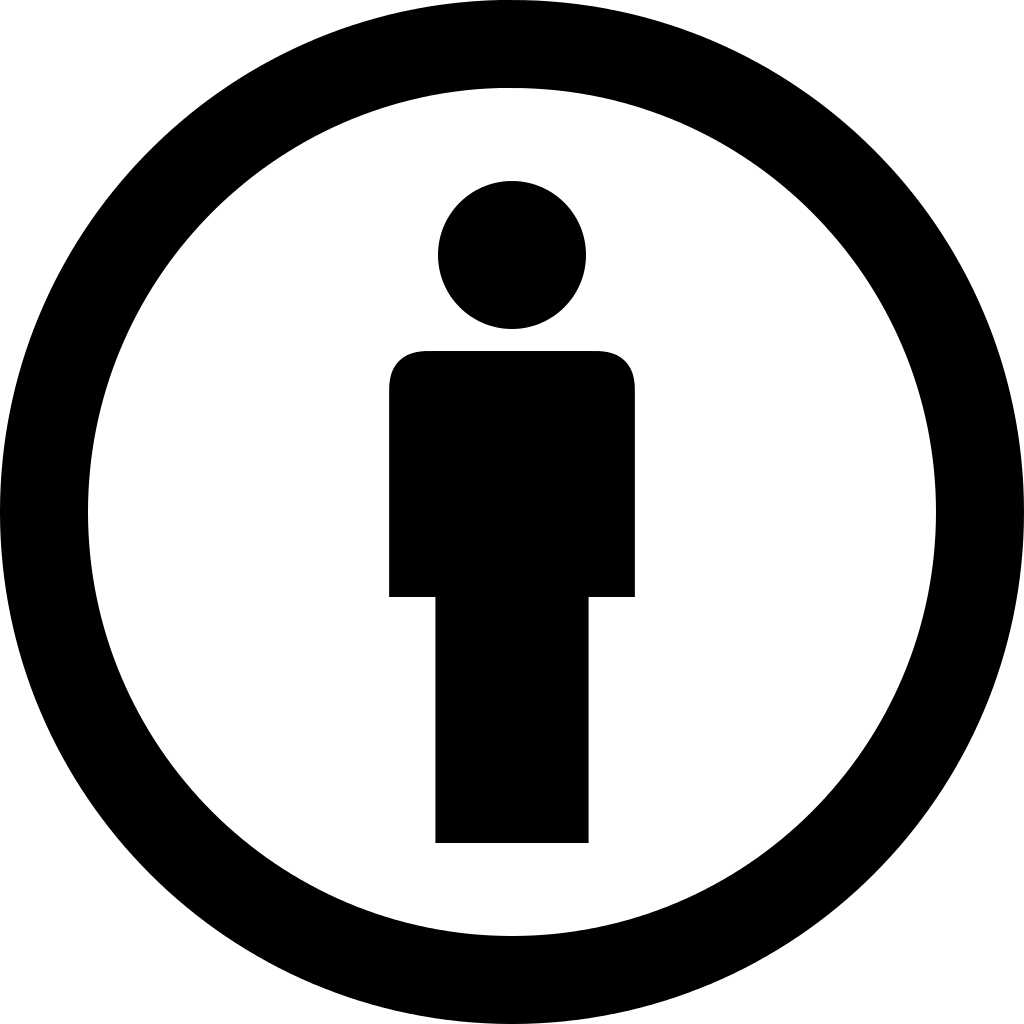
\includegraphics[width=0.2\textwidth]{BY.png}
    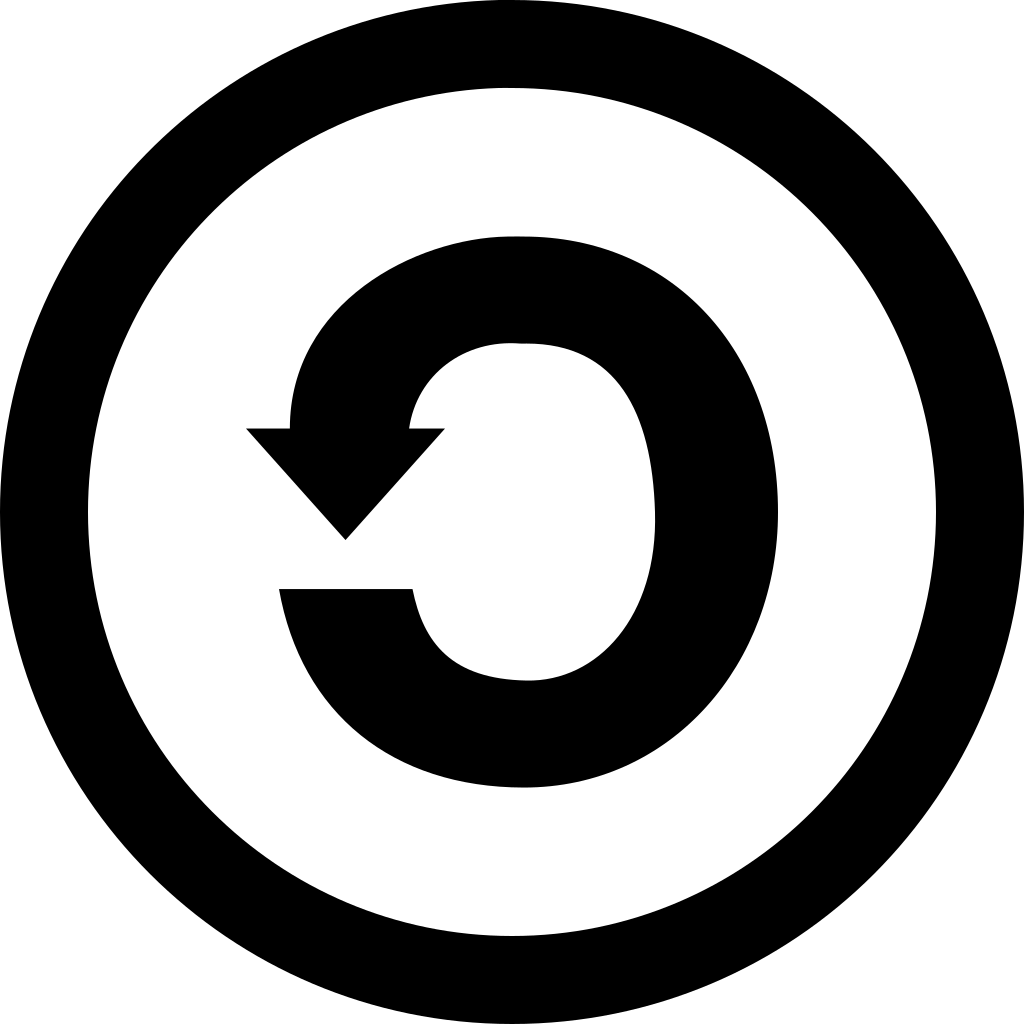
\includegraphics[width=0.2\textwidth]{SA.png}
  \end{center}

  This work is licensed under a
  \href{https://creativecommons.org/licenses/by-sa/4.0/}{Creative Commons
  Attribution-ShareAlike 4.0 International License}.
\end{frame}
\end{document}
